\documentclass[11pt,a4paper]{article}
\usepackage[margin=1in]{geometry}
\usepackage[T1]{fontenc}
\usepackage[utf8]{inputenc}
\usepackage{lmodern}
\usepackage{hyperref}
\usepackage{enumitem}
\usepackage{array}
\usepackage{longtable}
\usepackage{booktabs}
\usepackage{xurl}
\usepackage{tikz}
\usepackage{float}
\usetikzlibrary{arrows.meta, positioning, shapes.geometric}

\hypersetup{colorlinks=true,linkcolor=blue,urlcolor=blue}
\newcommand{\codepath}[1]{\path{#1}}
\setlength{\tabcolsep}{4pt}
\renewcommand{\arraystretch}{1.15}
\tikzset{
  box/.style={rectangle, draw, rounded corners, align=center, inner sep=3pt, minimum width=35mm},
  decision/.style={diamond, draw, aspect=2.2, align=center, inner sep=2pt},
  line/.style={-Latex}
}

\title{Document 1: Validation --- Phase-1}
\author{SIT Engine Architecture}
\date{\today}

\begin{document}
\maketitle
\tableofcontents
\newpage

\section{Purpose \& Scope}
\subsection*{Semantic Correctness in This Context}
Semantic correctness means the SIT outputs preserve engine behavior invariants, not only file-format validity. In Phase-1 this requires:
\begin{itemize}[leftmargin=*]
  \item resident-window SIT stays within physical bounds \([0,1]\),
  \item state fractions (\texttt{active\_frac}, \texttt{stall\_frac}, \texttt{idle\_frac}) conserve resident time,
  \item non-resident windows do not carry synthetic activity (\texttt{NaN} semantics),
  \item residency boundary behavior is exact for known edge modes (\texttt{skip\_w0}, \texttt{partial}, \texttt{exact\_boundary}).
\end{itemize}

\subsection*{Regressions the Suite is Designed to Catch}
\begin{itemize}[leftmargin=*]
  \item interval/window overlap regressions from time slicing changes,
  \item residency leakage where accumulation occurs outside residency masks,
  \item state accounting drift where fractions stop summing to one,
  \item output-field drift that breaks invariant evaluation assumptions.
\end{itemize}

\subsection*{Relationship to SIT Engine Core and Output Schema v1}
\begin{itemize}[leftmargin=*]
  \item Engine producer: \codepath{Phase-1/sit_engine_phase1.py}
  \item Phase-0 baseline context: Tenstorrent Wormhole testbench traces normalized via \codepath{Phase-1/phase0_trace_to_sit.py}
  \item Semantic validator: \codepath{Phase-1/tests/check_invariants.py}
  \item Golden replay orchestrator: \codepath{Phase-1/tests/run_golden_suite.py}
  \item Output contract authority: \codepath{Phase-1/schema/v1.py}
  \item Export integration point: \codepath{Phase-1/cli.py} (\texttt{cmd\_export})
\end{itemize}

\subsection*{Phase-0 Baseline Provenance (Verified)}
\begin{itemize}[leftmargin=*]
  \item Source repo: \url{git@github.com:Srinidhi-Magesh08/Tenstorrent_test_raw_files.git}
  \item Baseline branch/commit: \texttt{main} @ \texttt{4512ce4e1a689f64c866160bf1f8e7e5e3e2ec89}
  \item Baseline run artifact: \codepath{phase0_golden/tt_run_2026-02-09/raw_profiler/profile_log_device.csv}
  \item Run header baseline: \texttt{ARCH=wormhole\_b0}, \texttt{CHIP\_FREQ[MHz]=1000}, \texttt{Max Compute Cores=64}
\end{itemize}

\section{Architecture \& Components}
\subsection*{Validation Suite Structure}
\begin{itemize}[leftmargin=*]
  \item \textbf{Golden Orchestrator} (\codepath{tests/run_golden_suite.py}): loads manifest, runs engine per trace/mode, invokes invariants, aggregates failures.
  \item \textbf{Invariant Module} (\codepath{tests/check_invariants.py}): defines and enforces semantic invariants by mode.
  \item \textbf{Optional Trace Validator} (\codepath{tools/validation/validate.py}): operator-focused diagnostics over run artifacts (supplemental, not CI gate).
\end{itemize}

\subsection*{Golden Trace Execution and Comparison Model}
For each trace in \codepath{datasets/manifest.json}, the harness runs:
\begin{enumerate}[leftmargin=*]
  \item Base mode (no residency file).
  \item Residency modes (\texttt{all}, \texttt{skip\_w0}, \texttt{partial}, \texttt{exact\_boundary}) when masks exist.
  \item Invariant checks per generated \texttt{*\_windows.csv}.
\end{enumerate}
Model is invariant-first for the full dataset, with an explicit strict numeric parity gate for the Wormhole-derived Phase-0 sample via \codepath{tests/check\_phase0\_parity.py}.

\subsection*{Phase-0 Behavioral Truth Mapping (Authoritative)}
Converting Tenstorrent trace format alone is not sufficient. The mapping used in this repository is:
\begin{itemize}[leftmargin=*]
  \item Phase-0 reference defines expected engine decisions.
  \item Those decisions are encoded as golden assertions.
  \item Phase-1/Phase-2 runs must satisfy those assertions.
\end{itemize}

\textbf{Golden reference artifacts in repo:}
\begin{itemize}[leftmargin=*]
  \item TT-derived input trace: \codepath{datasets/traces/trace\_F\_phase0\_wormhole\_sample.csv}
  \item TT-derived expected engine outputs: \codepath{tests/fixtures/phase0\_parity\_expected.json}
\end{itemize}

\textbf{Requirement-to-validation mapping:}
\begin{itemize}[leftmargin=*]
  \item \textbf{Window boundary logic requirement:}
  Engine rule is fixed in \codepath{sit\_engine\_phase1.py} (\texttt{split\_interval\_into\_windows} with epsilon boundary handling); validated by strict row/value parity in \codepath{check\_phase0\_parity.py}.
  \item \textbf{Residency-gated accumulation requirement:}
  Engine intersection/gating logic is fixed in \codepath{sit\_engine\_phase1.py} (\texttt{intersect\_with\_mask}, resident accumulation); validated by parity fixture plus mode invariants in \codepath{check\_invariants.py} (\texttt{partial}, \texttt{exact\_boundary}, \texttt{skip\_w0}).
  \item \textbf{SIT computation requirement:}
  Engine SIT/fallback behavior is fixed in \codepath{sit\_engine\_phase1.py} (work-rate path and no-work fallback); validated through expected \texttt{sit} values in parity fixture via \codepath{check\_phase0\_parity.py}.
  \item \textbf{Output contract/stability requirement:}
  Expected summary/windows structure comes from parity fixture plus schema/invariant constraints; enforced by \codepath{run\_golden\_suite.py} orchestration.
\end{itemize}

\textbf{Phase mapping:}
\begin{itemize}[leftmargin=*]
  \item \textbf{Phase-1:} strict TT parity for \texttt{trace\_F} is mandatory (hard fail on mismatch or non-execution) in \codepath{run\_golden\_suite.py}.
  \item \textbf{Phase-2:} same engine is reused via \codepath{Phase-2/tests/run\_golden\_suite.py}; adapters map simulator markers into equivalent semantics, but strict TT numeric parity is not enabled by default.
\end{itemize}

\subsection*{Invariant Definitions (Code-Level)}
Common checks:
\begin{itemize}[leftmargin=*]
  \item \texttt{check\_sit\_bounds()}
  \item \texttt{check\_fracs\_sum\_to\_one()}
  \item \texttt{check\_nonresident\_are\_nan()}
\end{itemize}

Mode-specific checks:
\begin{itemize}[leftmargin=*]
  \item \texttt{check\_skip\_w0()}
  \item \texttt{check\_partial\_expected\_resident\_us()}
  \item \texttt{check\_exact\_boundary()}
\end{itemize}

\section{Implementation Detail}
\subsection*{File/Module Layout}
\begin{itemize}[leftmargin=*]
  \item \codepath{Phase-1/tests/run_golden_suite.py}
  \item \codepath{Phase-1/tests/check_invariants.py}
  \item \codepath{Phase-1/tests/check_phase0_parity.py}
  \item \codepath{Phase-1/tests/fixtures/phase0_parity_expected.json}
  \item \codepath{Phase-1/datasets/manifest.json}
  \item \codepath{Phase-1/sit_engine_phase1.py}
  \item \codepath{Phase-1/schema/v1.py}
  \item \codepath{Phase-1/cli.py}
\end{itemize}

\subsection*{How Checks are Registered and Triggered}
Registration is explicit dispatch (not plugin-based):
\begin{itemize}[leftmargin=*]
  \item \texttt{run\_golden\_suite.py} hardcodes mode map and shell-invokes engine + invariant script.
  \item \texttt{run\_golden\_suite.py} also invokes \texttt{check\_phase0\_parity.py} for \texttt{trace\_F\_phase0\_wormhole\_sample.csv} in base mode.
  \item Missing trace files, missing residency mask keys/files, or zero executed runs are treated as hard failures.
  \item \texttt{check\_invariants.py} selects mode-specific assertions via \texttt{--mode}.
\end{itemize}

\subsection*{Failure Reporting and Surface Area}
\begin{itemize}[leftmargin=*]
  \item Invariant failures raise \texttt{AssertionError}, print \texttt{FAIL: ...}, exit code 2.
  \item Golden harness aggregates \((trace, stage, output)\), prints consolidated failures, exits code 2.
  \item Non-zero exit propagates directly to CI job failure.
\end{itemize}

\section{CI Integration}
\subsection*{Hook Path}
\codepath{.github/workflows/phase1-ci.yml}

\subsection*{Trigger Conditions}
\begin{itemize}[leftmargin=*]
  \item \texttt{push} when changed paths include \texttt{Phase-1/**} or \texttt{.github/workflows/phase1-ci.yml},
  \item \texttt{pull\_request} with the same path filters,
  \item No nightly/scheduled trigger configured in current workflow.
\end{itemize}

\subsection*{How Semantic Drift Fails PRs}
CI runs \texttt{python tests/run\_golden\_suite.py --outdir /tmp/golden\_out\_ci}. Any invariant failure or Phase-0 parity mismatch produces non-zero exit, causing workflow failure and PR blocking.

\subsection*{Executed Cross-Checks and Python Test Runs}
The following script-driven validation checks were executed and passed in the current environment:
{\small
\begin{longtable}{@{}>{\raggedright\arraybackslash}p{0.56\textwidth} >{\centering\arraybackslash}p{0.08\textwidth} >{\raggedright\arraybackslash}p{0.30\textwidth}@{}}
\toprule
\textbf{Executed Command} & \textbf{Result} & \textbf{Evidence / Artifact} \\
\midrule
\endhead
\begin{tabular}[t]{@{}l@{}}\texttt{python3 tests/run\_golden\_suite.py}\\\texttt{--outdir /tmp/phase1\_golden\_with\_parity}\end{tabular} & PASS & \texttt{ALL PASS: golden suite} \\
\begin{tabular}[t]{@{}l@{}}\texttt{python3 tests/check\_phase0\_parity.py --windows}\\\texttt{/tmp/phase1\_golden\_with\_parity/trace\_F\_phase0\_wormhole\_sample\_\_}\\\texttt{base\_windows.csv --summary}\\\texttt{/tmp/phase1\_golden\_with\_parity/trace\_F\_phase0\_wormhole\_sample\_\_}\\\texttt{base\_summary.json}\end{tabular} & PASS & \texttt{PASS phase0 parity} \\
\begin{tabular}[t]{@{}l@{}}\texttt{python3.9 tests/run\_golden\_suite.py}\\\texttt{--outdir /tmp/phase1\_golden\_py39}\end{tabular} & PASS & 40 summaries generated\\(8 traces \(\times\) 5 modes) \\
\begin{tabular}[t]{@{}l@{}}\texttt{python3 cli.py ingest --trace}\\\texttt{datasets/traces/trace\_A\_single\_residency.csv --out}\\\texttt{/tmp/phase1\_export\_check}\end{tabular} & PASS & ingest smoke artifacts\\written \\
\texttt{python3 cli.py classify --in /tmp/phase1\_export\_check --window-us 256} & PASS & \texttt{windows.csv},\\\texttt{summary.json} emitted \\
\texttt{python3.9 cli.py export --in /tmp/phase1\_export\_check --schema v1} & PASS & \texttt{windows\_v1.csv},\\\texttt{summary\_v1.json},\\\texttt{windows\_v1.parquet} \\
\bottomrule
\end{longtable}
}

Validation metrics observed from \texttt{/tmp/phase1\_golden\_py39}:
\begin{longtable}{>{\raggedright\arraybackslash}p{0.22\textwidth} >{\raggedright\arraybackslash}p{0.18\textwidth} >{\raggedright\arraybackslash}p{0.18\textwidth} >{\raggedright\arraybackslash}p{0.28\textwidth}}
\toprule
\textbf{Mode} & \textbf{sit\_median avg} & \textbf{sit\_p95 avg} & \textbf{resident\_windows\_total avg} \\
\midrule
\endhead
\texttt{base} & 0.5757 & 0.5757 & 5.25 \\
\texttt{partial} & 0.1840 & 0.1840 & 12.00 \\
\texttt{exact\_boundary} & 0.1819 & 0.1819 & 4.00 \\
\texttt{all} & 0.0001 & 0.0001 & 31252.00 \\
\texttt{skip\_w0} & 0.0001 & 0.0001 & 31248.00 \\
\bottomrule
\end{longtable}

Test framework note: current repository validation is script-driven (\texttt{run\_golden\_suite.py}, \texttt{check\_invariants.py}); there is no pytest test-discovery suite in the current codebase.

\section{Flowchart}
\begin{figure}[H]
  \centering
  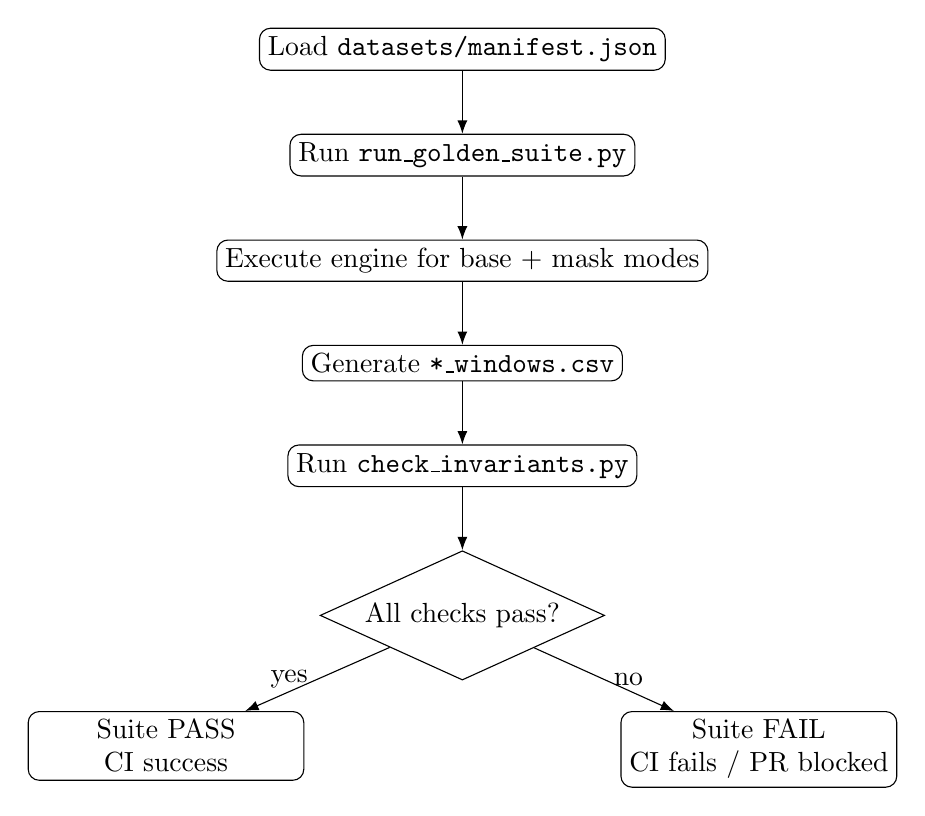
\begin{tikzpicture}[node distance=8mm and 11mm]
    \node[box] (m) {Load \texttt{datasets/manifest.json}};
    \node[box, below=of m] (g) {Run \texttt{run\_golden\_suite.py}};
    \node[box, below=of g] (e) {Execute engine for base + mask modes};
    \node[box, below=of e] (w) {Generate \texttt{*\_windows.csv}};
    \node[box, below=of w] (i) {Run \texttt{check\_invariants.py}};
    \node[decision, below=of i] (d) {All checks pass?};
    \node[box, below left=of d] (p) {Suite PASS\\CI success};
    \node[box, below right=of d] (f) {Suite FAIL\\CI fails / PR blocked};
    \draw[line] (m) -- (g);
    \draw[line] (g) -- (e);
    \draw[line] (e) -- (w);
    \draw[line] (w) -- (i);
    \draw[line] (i) -- (d);
    \draw[line] (d) -- node[left]{yes} (p);
    \draw[line] (d) -- node[right]{no} (f);
  \end{tikzpicture}
  \caption{Validation Flow: Golden Replay to CI Verdict}
\end{figure}

\section{Done-When Criteria Mapping}
Done-when target: \textbf{CI detects semantic regressions.}

\begin{longtable}{@{}>{\raggedright\arraybackslash}p{0.27\textwidth} >{\raggedright\arraybackslash}p{0.29\textwidth} >{\raggedright\arraybackslash}p{0.40\textwidth}@{}}
\toprule
\textbf{Invariant / Gate} & \textbf{Code Path} & \textbf{Done-When Contribution} \\
\midrule
\endhead
SIT bounds (\(0 \le sit \le 1\)) & \codepath{check_sit_bounds} & Detects normalization drift and impossible throughput values. \\
Fraction conservation & \codepath{check_fracs_sum_to_one} & Detects state accounting overlap/gap regressions. \\
Non-resident NaN discipline & \codepath{check_nonresident_are_nan} & Detects accumulation leakage outside residency. \\
Skip first window behavior & \codepath{check_skip_w0} & Detects window-index boundary drift. \\
Partial overlap arithmetic & \codepath{check_partial_expected_resident_us} & Detects partial-window overlap math regressions. \\
Exact boundary semantics & \codepath{check_exact_boundary} & Detects boundary double-count/misassignment regressions. \\
Phase-0 strict parity gate & \codepath{check_phase0_parity.py} & Detects numeric drift against the pinned Wormhole-derived baseline sample output. \\
Dataset-wide harness & \codepath{run_golden_suite.py} & Scales checks across all traces/masks and fails on any semantic violation. \\
CI workflow execution & \codepath{phase1-ci.yml} & Enforces regression detection on PR and push events. \\
\bottomrule
\end{longtable}

\end{document}
